
正如记录需求一样,也应该记录出现的架构。这当然不仅仅是为了拥有文档,它应该帮助每个参与项目的人提高生产力,使他们更好地理解自己的角色和最终产品需要什么。并不是所有的图表都对每个人都有用,但是可以试着从未来读者的角度来创建它们。

有许多框架可以记录愿景,其中许多框架服务于特定的领域、项目类型或体系结构范围。例如,如果对记录企业架构感兴趣,那么可能会对TOGAF感兴趣。这是\textit{开放组架构框架}的首字母缩写。它依赖于四个领域,即:

\begin{itemize}
\item 
业务架构(策略、组织、关键流程和治理)

\item 
数据架构(逻辑和物理数据管理)

\item 
应用架构(单系统的蓝图)

\item
技术架构(硬件、软件和网络基础设施)
\end{itemize}

如果将软件记录放在整个公司,甚至更广泛的范围内,那么这种分组就很重要。其他类似规模的框架包括由\textbf{英国国防部(MODAF)}和\textbf{美国等效机构(DoDAF)}开发的框架。

如果没有记录企业架构,若是刚刚开始架构自我开发道路,可能会对其他框架更感兴趣,例如4+1和C4模型。

\subsubsubsection{3.6.1\hspace{0.2cm}4+1模型}

4+1模型是由Philippe Kruchten在1995年创建,作者称它旨在“对多个并发视图的使用,描述软件密集型系统的架构”。它的名字来自于它所包含的视图。

这种模型已经在市场上存在了很长时间,也非常有效果,因此广为人知。它非常适合于大项目,当然也可以用于中小型的项目,但对于需求来说也可能过于复杂(特别是用敏捷的方式编写的)。如果正处于这种情况,应该尝试下一节中的C4模型。

4+1模型的缺点是它使用了一组固定的视图,而文档体系结构需要根据项目的具体情况选择视图(稍后将详细介绍)。

优点是可以清晰的了解视图是如何连接在一起,特别是涉及到场景时。同时,每个责任方可以很容易地了解与他们相关的部分。

\begin{center}
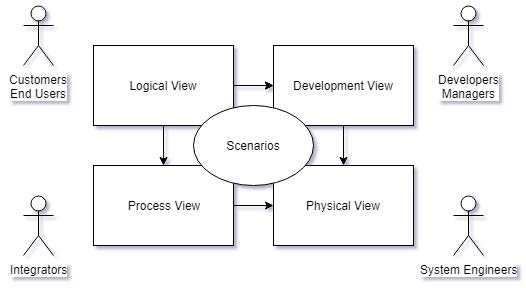
\includegraphics[width=0.6\textwidth]{content/1/chapter3/images/1.jpg}\\
图3.1 - 4+1模式概览
\end{center}

上图中的参与者对其对应的视图最感兴趣,所有的视图都可以用不同种类的\textbf{统一建模语言(UML)}图来表示。先了解下每个视图:

\begin{itemize}
\item 
\textbf{逻辑视图}展示了如何向用户提供功能,以及系统的组件(对象)如何交互。最常见的是,由类和状态图组成。如果有成千上万的类或者只是想更好地显示交互,应该有通信图或序列图,两者都是下个视图的一部分:

\begin{center}
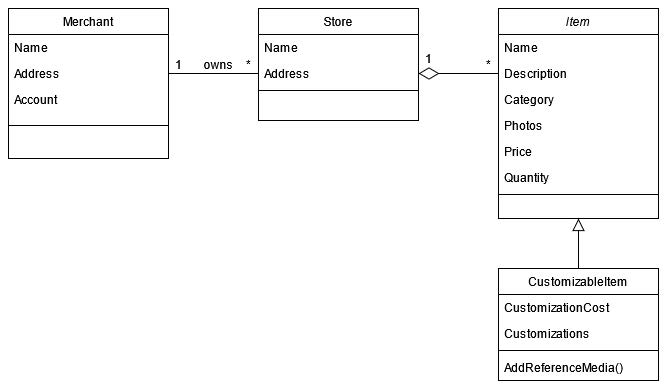
\includegraphics[width=0.7\textwidth]{content/1/chapter3/images/2.jpg}\\
图3.2 -类图可以用来显示计划拥有的类型,以及它们的关系
\end{center}

\item 
\textbf{进程视图}围绕着系统的运行时行为,显示进程、进程之间的通信以及与外部系统的交互,由活动和交互图表示。此视图处理许多NFR,包括并发性、性能、可用性和可扩展性:

\begin{center}
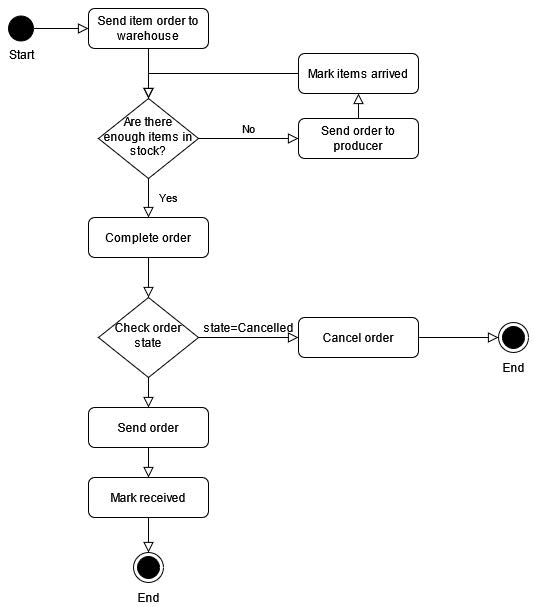
\includegraphics[width=0.6\textwidth]{content/1/chapter3/images/3.jpg}\\
图3.3 -活动图工作流和过程的图形表示
\end{center}

\item 
\textbf{开发视图}为了分解成子系统,并围绕着软件组织。重用、工具约束、分层、模块化、打包、执行环境——这个视图可以通过显示系统的构建块来表示。通过使用组件和包图来实现:

\begin{center}
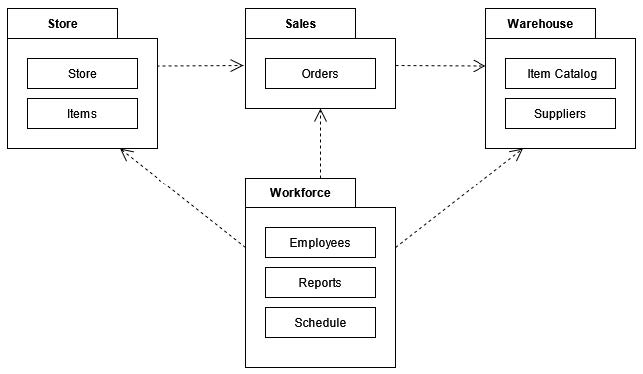
\includegraphics[width=0.8\textwidth]{content/1/chapter3/images/4.jpg}\\
图3.4 -包图可以从更高的角度显示系统的各个部分,以及特定组件之间的依赖关系
\end{center}

\item
\textbf{物理视图}使用部署图将软件映射到硬件。针对系统工程师,可以涵盖与硬件相关的NFR子集,例如通信:

\begin{center}
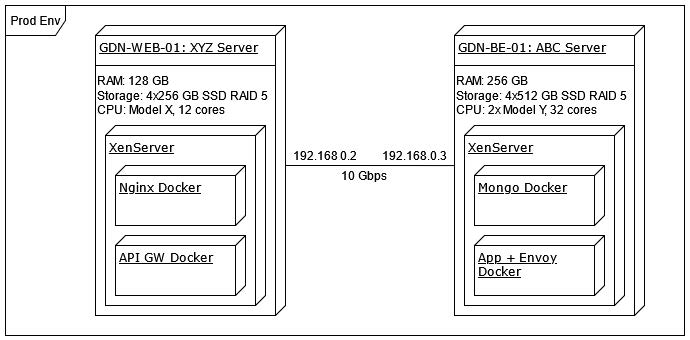
\includegraphics[width=0.9\textwidth]{content/1/chapter3/images/5.jpg}\\
图3.5 -部署图展示了运行每个软件组件的硬件,还可以用来传递有关网络的信息
\end{center}

\item
\textbf{场景视图}把所有其他的视图都连接在一起,这些对所有相关方都是有用的。这个视图可以显示系统是否做了它应该做的事情。当其他视图都完成后,场景视图可能是多余的。但是,如果没有使用场景,其他视图都是不可能完成。这个视图从高层次展示了系统,而其他视图则展示了更多的细节:

\begin{center}
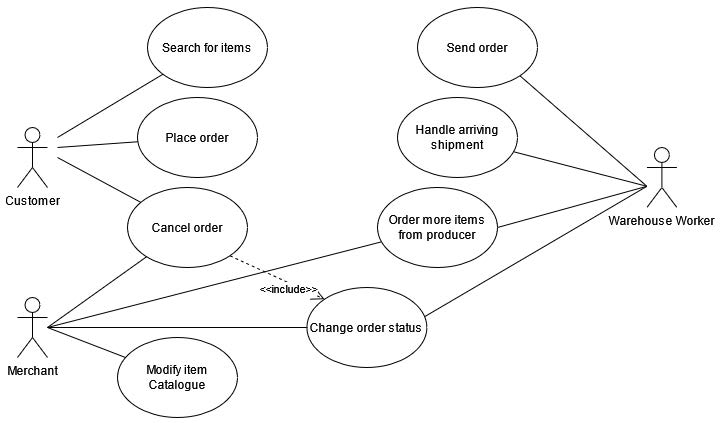
\includegraphics[width=0.9\textwidth]{content/1/chapter3/images/6.jpg}\\
图3.6 -用例图显示了特定的参与者如何与系统交互,以及如何交互,彼此关联
\end{center}

\end{itemize}

这些视图中的每一个都与其他视图相互关联,才能显示出全貌。这里需要考虑下,如何表达并发。它不能只使用逻辑视图来完成,因为将其映射到任务和流程更有表现力,从而需要过程视图。另一方面,进程将映射到物理(通常是分布式的)节点。这意味着需要在三个视图中进行记录,每个视图都与特定的责任方相关。视图之间的其他连接包括:

\begin{itemize}
\item
逻辑视图和过程视图都用于分析和设计,以概念化产品。

\item 
将开发和部署放在一起,描述了软件是如何打包的,以及每个包将在何时部署。

\item
逻辑视图和开发视图显示了功能如何反映在源码中。

\item
流程和部署视图共同描述NFR。
\end{itemize}

熟悉了4+1模型,继续了解另一个简单但非常有效的模型:C4模型。希望它的使用过程充满了爆炸性(双关语[译注:关联的是著名的C4炸弹])。

\subsubsubsection{3.6.2\hspace{0.2cm}C4模型}

C4模型非常适合中小型项目。因为简单,所以易应,并且不依赖于任何预定义的符号。如果想用它来绘制图表,可以试试Tobias Shochguertel的c4-draw.io插件(\url{https://github.com/tobiashochguertel/c4-draw.io})的免费在线绘图工具-draw.io(\url{https://www.draw.io/})。

C4模型中,主要有四种图类型,即:

\begin{itemize}
\item
系统上下文

\item 
容器

\item
组件

\item
代码
\end{itemize}

就像使用地图放大和缩小一样,可以使用这四种类型来显示特定代码区域的细节,或者“缩小”来显示关于特定模块,甚至整个系统的交互和周围环境的更多信息。

系统上下文是查看架构的一个很好的起点,因为它将系统作为一个整体显示出来,周围是与其交互的用户和其他系统。可以在这里看到一个C4模型的上下文关系图:

\begin{center}
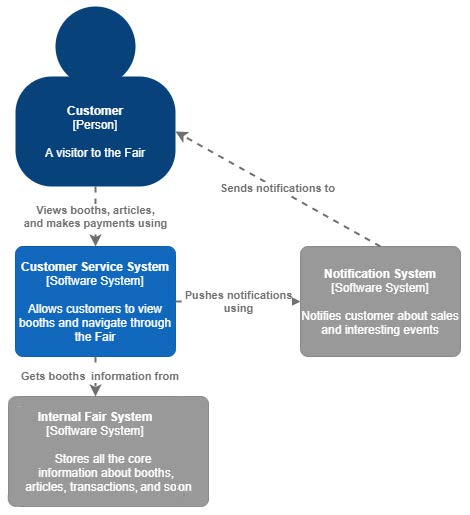
\includegraphics[width=0.6\textwidth]{content/1/chapter3/images/7.jpg}\\
图3.7 - C4上下文关系图
\end{center}

它展示了“大局”,所以它不应该专注于特定的技术或协议。相反,可以把它看作是可以向非技术相关方展示的图表。仅通过查看图表,就可以清楚地看到有一个参与者(对客户的人形描述),他与解决方案的一个组件(即客户服务系统)交互。另一方面,这个系统与另外两个系统相互作用,每个相互作用都用箭头表示。

上下文关系图用于提供系统的概览,其中包含一些细节。现在看下其他图表:

\begin{itemize}
\item
\textbf{容器图}: 用来显示系统内部的概述。如果系统使用数据库,提供服务,或者只是由某些应用程序组成,则此图将显示它。还可以展示容器的主要技术选择。注意,容器不是指Docker容器,尽管每个图都是单独的可运行和部署单元,但此图类型与部署场景无关。容器视图是为技术人员设计的,但并不仅限于开发团队。架构师以及操作和支持人员也是目标受众。

\item 
\textbf{组件图}: 如果想要关于特定容器的更多细节信息,就需要组件图发挥作用了。它展示了所选容器内的组件如何彼此交互,以及如何与容器外的元素和参与者交互。通过查看这张图,可以了解每个组件的职责,以及使用什么技术构建。组件图的目标受众主要集中在一个特定的容器上,由开发团队和架构师组成。

\item
\textbf{代码图}: 最后来看代码图,将组件放大到一定程度时,代码图就会出现。这个视图主要由UML图组成,包括类、实体关系和其他,理想情况下应该由独立的工具和IDE从源代码自动创建。不应该为系统中的每个组件制作这样的关系图;相反,把重点放在最重要的内容上,让它们告诉读者架构想要表达的内容。想要这样的图中少一些,就要从代码图中删掉不必要的元素。在许多系统中,特别是在较小的系统中,这类图会直接省略。
\end{itemize}

细心地读者可能会发现C4模型缺少一些特定的视图。例如,想知道如何演示应该如何部署系统,可能会有兴趣了解除了主图之外,还有一些补充图。其中之一是部署图,展示了如何将系统中的容器映射到基础设施中的节点。通常,其是UML部署图的简化版本:

\begin{center}
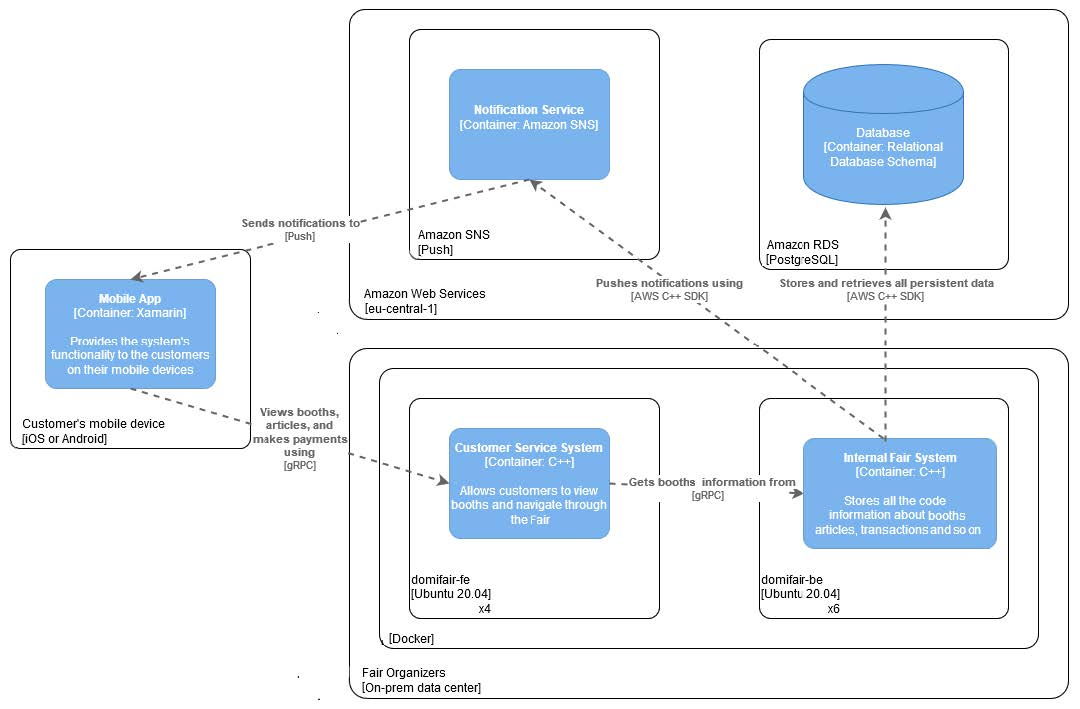
\includegraphics[width=0.9\textwidth]{content/1/chapter3/images/8.jpg}\\
图3.8 - C4部署图
\end{center}

说到与C4模型相关的UML图,可能还要知道为什么它在展示系统的用例上投入的这么少。如果遇到了这种情况,应该考虑使用UML的用例图来补充前面的模型,或者可能考虑引入一些序列图。

记录架构时,记录的内容和共享的知识比遵循硬性规则更重要,可以选择最适合的工具。

\subsubsubsection{3.6.3\hspace{0.2cm}记录敏捷项目中的架构}

敏捷环境中,记录架构的方法应该与记录需求的方法类似。首先,考虑谁会阅读这些材料,确保以正确的方式描述了正确的事情。文档不需要冗长的Word文档,当有人描述架构时,可以使用演示文稿、Wiki页面、单个图表,甚至是会议的录音进行记录。

重要的是收集关于文档化架构的反馈。与文档化的需求一样,需要告知相关方文档的更新,以便大家了解都改进了哪里。尽管这看起来像是在浪费时间,但如果处理得当,会节省交付产品的时间。足够好的文档可以帮助新手快速上手工作,并指导不熟悉框架的责任人。如果只是在一些会议上讨论架构,那么很可能会议之后就没有人会记得出于什么原因才做出的那些决策,以及这些决策在不断变化的敏捷环境中是否仍然有效。

创建文档时,重复阅读很重要,因为很可能会对一两个重要的细节有一些误解。架构师或相关方负责人会了解更多的细节,从而对原有的决定进行更改。在文件认为是成熟和完成之前,至少要把准备好的文档多看几遍。通常,通过即时通讯工具、电话或面对面的交谈可以更快地完成任务,并解决可能出现的后续问题,所以比起电子邮件或其他异步的沟通方式,架构师可能会更喜欢这种方式。


























